 
\documentclass[12pt,a4paper,fleqn]{tufte-handout}    
\usepackage{graphicx}    
\usepackage{morefloats}    
\usepackage{amsmath}    
\usepackage{amssymb}    
\usepackage{rotating}    
% mcode options for matlab code insertion bw (for printing), numbered (line numbers), framed (frame around code blocks), useliterate (convert Matlab expressions to Latex ones), autolinebreaks (automatic code wraping, use it with caution    
\usepackage[literate]{mcode}    
\graphicspath{{figures/}{tex/}{../figures/}{../../}{../}}     
\title{soundProjection}    
\author{ Mathieu Lagrange }    
 
\begin{document}    
 
\maketitle    
 
Voici les resultats de mon etude sur les projections alternatives a mds.   
 
 
 
% Please use this file to document your experiment    
% You can compile the report by setting the option 'report' as detailed in your expLanes configuration file.    
\begin{figure}   
\begin{center}   
\includegraphics[scale=.5]{figures/urban_pca}   
\caption{urban pca}   
\end{center}   
\end{figure}   
 
\begin{figure}   
\begin{center}   
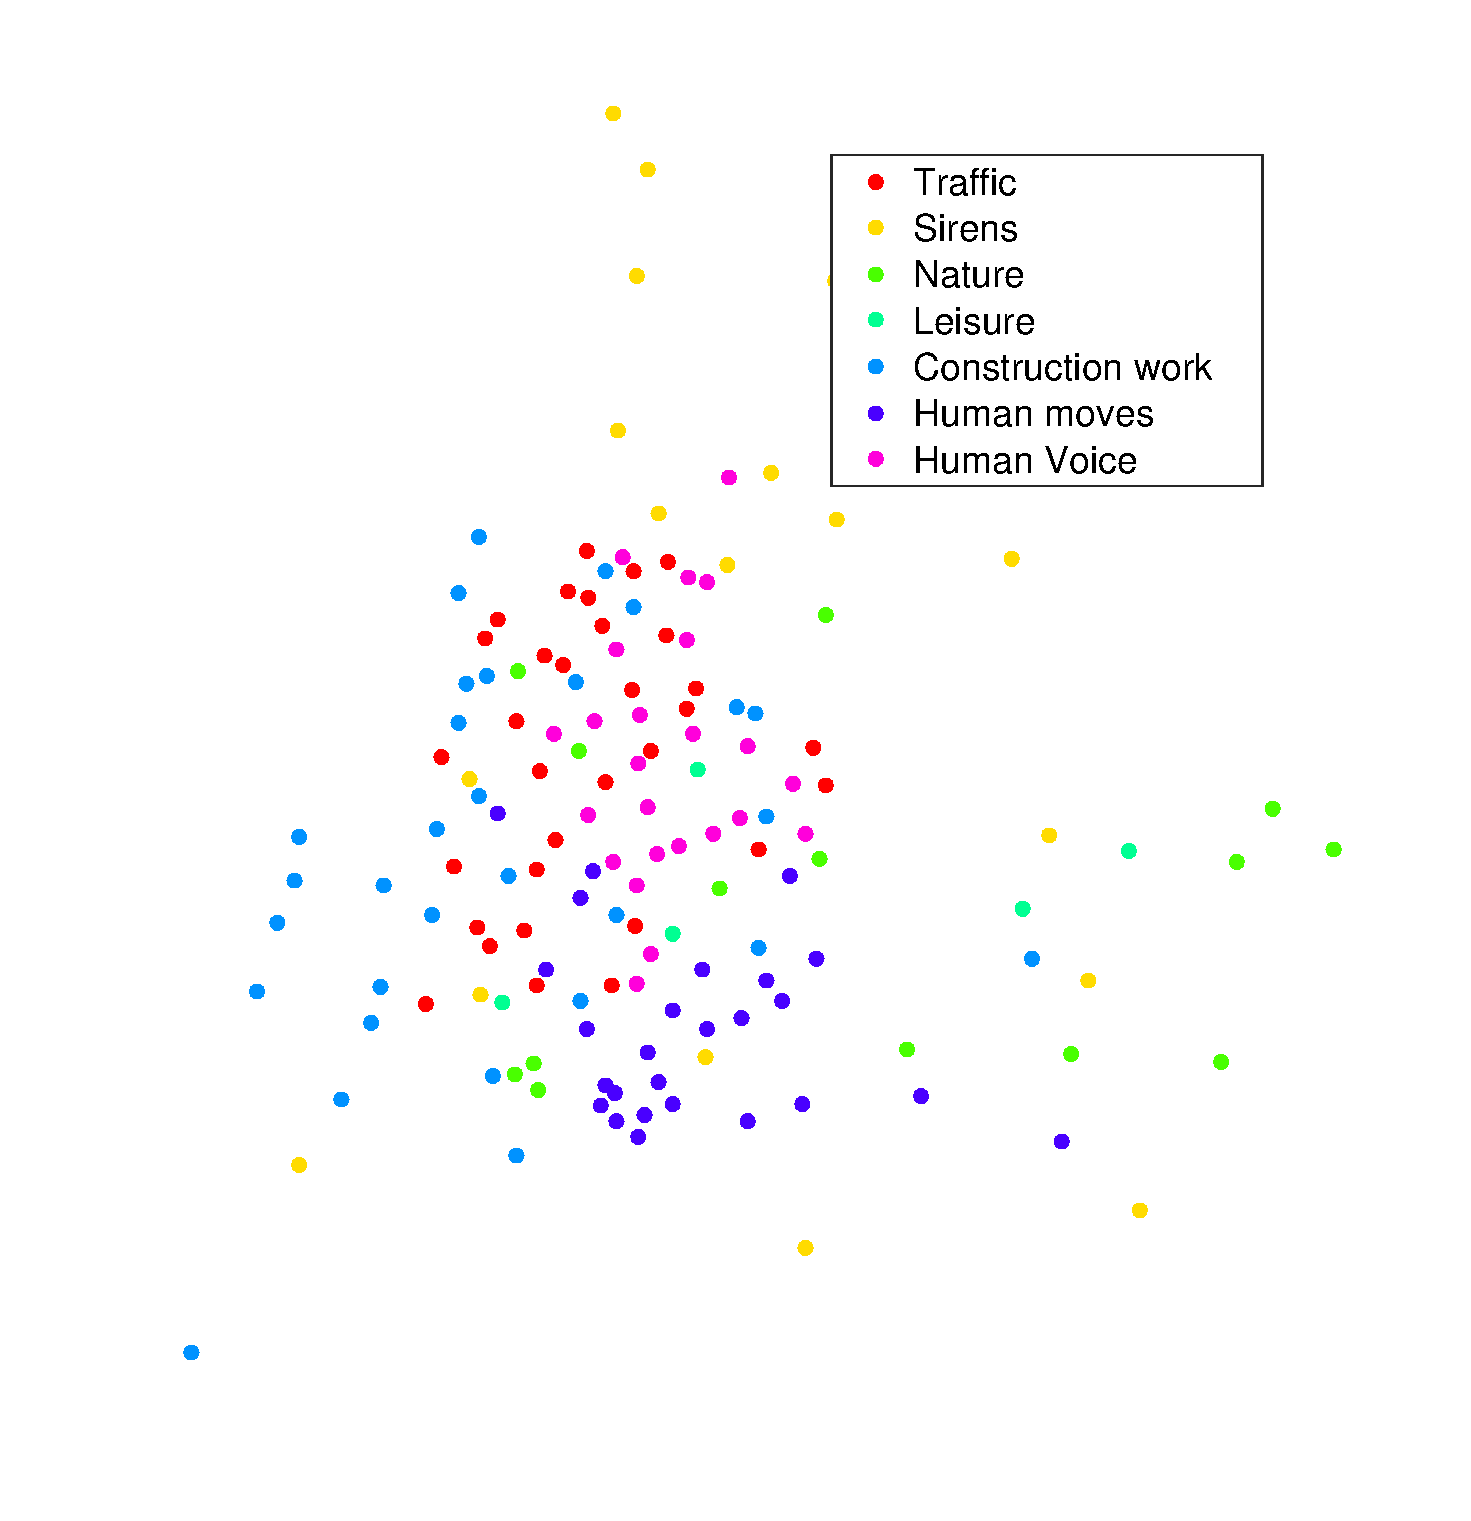
\includegraphics[scale=.5]{figures/urban_mds}   
\caption{urban mds}   
\end{center}   
\end{figure}   
 
\begin{figure}   
\begin{center}   
\includegraphics[scale=.5]{figures/urban_som}   
\caption{urban som}   
\end{center}   
\end{figure}   
 
\begin{figure}   
\begin{center}   
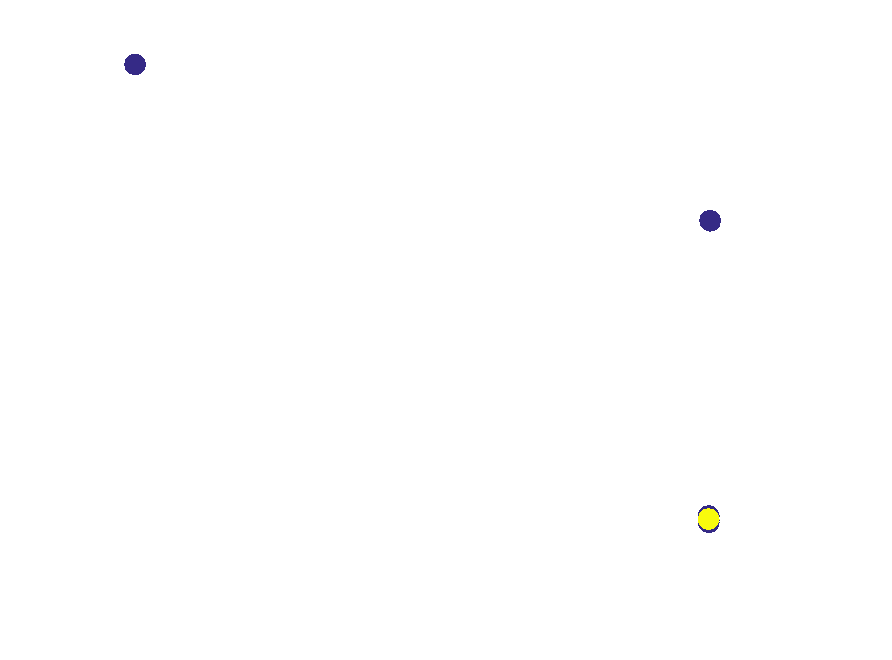
\includegraphics[scale=.5]{figures/music_pca}   
\caption{music pca}   
\end{center}   
\end{figure}   
 
\begin{figure}   
\begin{center}   
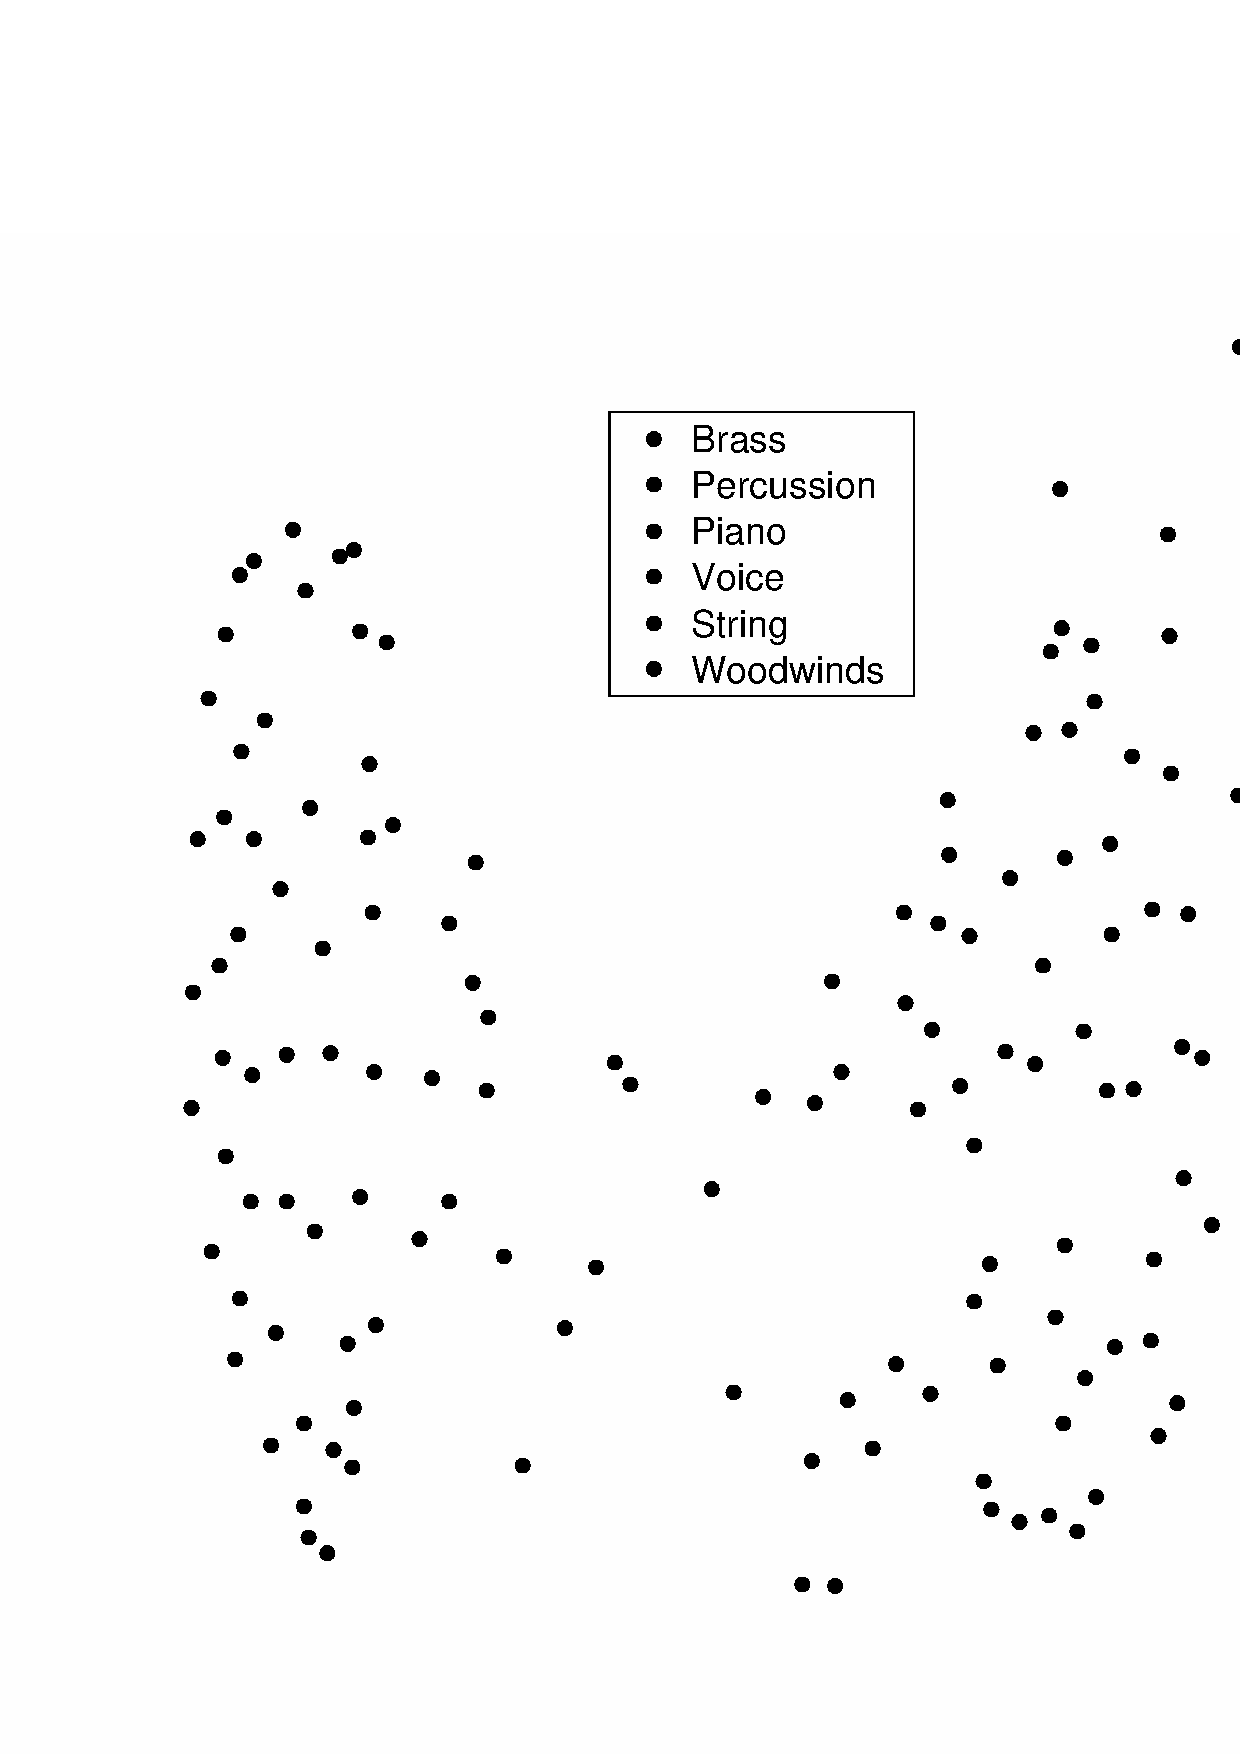
\includegraphics[scale=.5]{figures/music_mds}   
\caption{music mds}   
\end{center}   
\end{figure}   
 
\begin{figure}   
\begin{center}   
\includegraphics[scale=.5]{figures/music_som}   
\caption{music som}   
\end{center}   
\end{figure}   
 
 
 
 
 
 
\begin{table}  
\begin{center}  
\  
\setlength{\tabcolsep}{.16667em}  
\begin{tabular}{lcc}  
projection & meanAveragePrecision & precisionAt5 \\  
\hline  
som & 0.41 & 0.56 \\  
id & \textbf{\textcolor{red}{0.42}} & \textbf{\textcolor{red}{0.58}} \\  
pca & 0.29 & 0.21 \\  
mds & 0.38 & 0.50 \\  
\end{tabular}  
\end{center}  
\caption{database: urban, neurons: 9, spread: 0.5, nbRuns: 1}  
\label{daurNe9Sp0.5Nbru1}  
\end{table}  
 
  
\begin{table} 
\begin{center} 
\ 
 \setlength{\tabcolsep}{.16667em} 
\begin{tabular}{lcc} 
projection & meanAveragePrecision & precisionAt5 \\ 
\hline 
som & 0.40 & 0.47 \\ 
id & \textbf{\textcolor{red}{0.41}} & \textbf{\textcolor{red}{0.48}} \\ 
pca & 0.24 & 0.17 \\ 
mds & 0.39 & 0.42 \\ 
\end{tabular} 
\end{center} 
\caption{database: music, neurons: 9, spread: 0.5, nbRuns: 1} 
\label{damuNe9Sp0.5Nbru1} 
\end{table} 
 
  
 
  
  
\begin{table} 
\begin{center} 
\ 
 \setlength{\tabcolsep}{.16667em} 
\begin{tabular}{lcc} 
projection & meanAveragePrecision & precisionAt5 \\ 
\hline 
som & 0.41 & 0.56 \\ 
id & \textbf{\textcolor{red}{0.42}} & \textbf{\textcolor{red}{0.58}} \\ 
pca & 0.29 & 0.21 \\ 
mds & 0.38 & 0.50 \\ 
\end{tabular} 
\end{center} 
\caption{database: urban, neurons: 9, spread: 0.5, nbRuns: 1} 
\label{daurNe9Sp0.5Nbru1} 
\end{table} 
 
  
\begin{table} 
\begin{center} 
\ 
 \setlength{\tabcolsep}{.16667em} 
\begin{tabular}{lcc} 
projection & meanAveragePrecision & precisionAt5 \\ 
\hline 
som & 0.40 & 0.47 \\ 
id & \textbf{\textcolor{red}{0.41}} & \textbf{\textcolor{red}{0.48}} \\ 
pca & 0.24 & 0.17 \\ 
mds & 0.39 & 0.42 \\ 
\end{tabular} 
\end{center} 
\caption{database: music, neurons: 9, spread: 0.5, nbRuns: 1} 
\label{damuNe9Sp0.5Nbru1} 
\end{table} 
 
 % expLanesInsertionFlag DO NOT CLEAR (but move it where you want the generated temporary LaTEX code to be inserted) 
 
 
\bibliographystyle{abbrvnat}    
\bibliography{bib}    
 
\end{document}    
